\documentclass {article}
\usepackage{cite}
\usepackage{fullpage}
\usepackage{etoolbox}
\usepackage{url}
\usepackage{amsmath}
\usepackage{graphicx}
\usepackage{float}

\setlength\parindent{24pt}
\begin{document}

~\vfill
\begin{center}
\Large

Final Project - A5

Photorealistic Minecraft Ray Tracer

Qiuhan (Leo) Wang

Student ID: 20710836

User ID: q349wang
\end{center}
\vfill ~\vfill~
\newpage
\section{Purpose}
Minecraft is a popular sandbox survival game known for its cubic models
and pixel art design \cite{Minecraft}. While this design does have it's novelty, the rendering
engine it uses is very simple and does not create high-quality realistic scenery. 
The purpose of this project is to create a raytracer that is
capable of rendering photorealistic depictions of a handcrafted Minecraft scene 
consisting of various Minecraft blocks and objects.
\section{Statement}
This project is a raytracer that can be used to render various different scenes
using several different graphics techniques to achieve a photorealistic effect. Ultimately, 
the end goal of this project is to use these techniques to render a custom Minecraft scene
that looks like it could exist in real life.\medskip
\par
The final scene that will be rendered is a depiction of a Minecraft world that
I built. In this Minecraft world, there will be a small 1 room wooden
house situated on hill. The house will have a door at the front and large windows on the
other three walls. Inside of the
house will be a table as well as some common Minecraft blocks such as
a crafting table, an anvil, a chest and a furnace. The interior will be lit up by torches as well
the glow from the furnace. On the table will be several objects. These objects
are a potion bottle, a blaze rod, an ender pearl, a iron pickaxe and a gold ingot.
The sky will be dark like night time and stars should be visible. This scene
will be visible from multiple view points to illustrate both the interior and exterior
details of the environment.

\par
Since this is a raytracer, it will be building off the code I wrote
in Assignment 4. In Assignment 4, the extra objective that I intend to complete is anti-aliasing
via supersampling. As such that will not need to be implemented again. Instead, 
what needs to be done is implementing the new features of the raytracer that are requesting
in the objectives. These are reflection, transmission, texture mapping, bump mapping, depth
of field, photon mapping and environment mapping. In addition, 
new models and scenes will need
to be created to test these features as well as to construct the final Minecraft scene. To
fully capture the final scene, several camera positions will be required as well, thus
need to be supported by the raytracer.
\par
There are several interesting challenges that will need to be overcome in this project.
The largest challenge will be to properly implement an efficient photon mapping algorithm. 
There are many factors here to consider such as the memory usage of the algorithm
as well as the speed. Too much memory usage and I will not be able to map enough photons
for the rendered scene.
Too slow and I will run out of time trying to render the scene. Trying to 
create the models and scenes will also be interesting. Since most of Minecraft's
objects are 2D sprites, I will need to determine how to accurately create their 3D representations
as models to be placed in the scene. Finally,
Minecraft is a game that I've been playing since I was a kid, and I'd love to 
see how realistic Minecraft would look if it used more advanced rendering techniques.
\par
The main takeaways from this project will be the proper implementation details
of the many advanced rendering and modelling features used in this raytracer. Hopefully, by
reading through the various articles on these topics and by
programming these myself, I can gain a deeper understanding of the techniques
used to produce realistic graphics as well as the optimizations and tradeoffs
utilized to achieve these efficiently.
\section{Objectives}
This section will review the objectives I proposed which I have completed in this project. They are as follows.
\begin{enumerate}
    \item Specular Reflection
    \item Specular Transmission
    \item Texture Mapping
    \item Bump Mapping
    \item Depth of Field
    \item Photon Map - Mapping
    \item Photon Map - Caustics
    \item Environment Mapping
    \item Minecraft Models
    \item Final Scene
\end{enumerate}

\section{Manual}
This section will go into detail regarding how each to use each of the new implemented 
features of the raytracer. It will cover how to compile and run the program as well
as important files related to each objective.
\subsection{Compilation}
This raytracer makes use of some of the shared libraries from previous assignments. As a result, 
the folder \textbf{A5} must be placed in the \textbf{cs488} directory where all the other assignments
exist. Similarly to the other assignments, to compile the program for the first time, change directories
to \textbf{cs488} and run 
\begin{verbatim}
    $ premake4 gmake
    $ make
\end{verbatim}
After this step,
change directories to \textbf{A5} and run
\begin{verbatim}
    $ premake4 gmake
    $ make config=release
\end{verbatim}
Ensure that the config is set to release as this will apply compiler optimizations which are highly desired.
This program was tested to work on WSL2 (Ubuntu 20.04.1 LTS) and should work on other
Linux machines as long as the appropriate libraries
are available. Once the program is compiled, the executable can be run with the following command where
\texttt{args} are command line arguments.
\begin{verbatim}
    $ ./FinalProgram <args>
\end{verbatim}
Ensure that the directory that the executable is running is is \textbf{A5} as this is important for proper
loading of assets and scripts. From this point forward, when we refer to a file or directory, we will
use its relative path from this directory.
\subsection{Command Line Interface}
Similarly to the A4 raytracer, this program takes in a file as its first argument at all times.
This file is a lua script which describes the scene geometry, lighting and parameters that
will be necessary for rendering. Many of the features can be enabled or disabled through the command line. This is
to allow for isolated testing and faster iteration as I could disable some performance
heavy features when only certain behaviour is desired. When a program is run, the current
state of the command arguments are outputted to the user in the terminal. Below is a 
This information can also be found in in the file \texttt{CMDArgs.hpp}.
\begin{enumerate}
    \item antialias (flag: -a) : If specified, anti-aliasing will be enabled
    \item drawAABB (flag: -b) : If specified, meshes will draw bounding boxes instead of triangles
    \item maxDepth (flag: -d x) : If specified, the maximum depth of path tracing is x. The default is 10
    \item phongShading (flag: -P) : If specified, normals for meshes will be interpolated from the vertices and shading will be smooth
    \item renderPhotonMap (flag: -p) : If specified, the raytracer will render the photon map created by the mapping objective instead of the scene
    \item renderCaustics (flag: -c) : If specified, the raytracer will generate a caustic photon map. If used in tandem with -p, will render the caustic
    photon map instead of the global photon map.
    \item numThreads (-t x) : If specified, will start the raytracer with x concurrent threads.
\end{enumerate}
Some sample executions of this program are as follows:
\begin{verbatim}
    $ ./FinalProgram Assets/simple.lua                  # Render scene with default config
    $ ./FinalProgram Assets/simple.lua -a               # Render scene with anti-aliasing
    $ ./FinalProgram Assets/simple.lua -p -c            # Render photon map with only caustic map photons
    $ ./FinalProgram Assets/simple.lua -c -P -t 9       # Render scene with caustics and Phong shading on at most 9 threads
\end{verbatim}
\subsection{Scripting Extensions}
Some of the features required extensions to the lua scripting library to properly function as they
modified dynamic parts of the scene. This section will detail the changes made as well as the proper 
method of using the new extensions. All of these extensions were added to scene\_lua.cpp
\subsubsection{gr.material Extensions} \label{material_ext}
To incorporate specular reflection and specular transmission, new material properties needed 
to added so that one can control the various properties related to these, such as the index
of refraction or the degree of reflectivity. These are implemented in a new material called DielectricMaterial
which will be discussed in the Implementation section. In the lua script, the \texttt{gr.material}
function is extended so that it can accommodate 3 more parameters optionally: a 3D vector for
specular reflectivity, a 3D vector for transmission, and an index of refraction number value. This gives the 
scripter the ability to call
\begin{verbatim}
gr.material({kdx, kdy, kdz}, {ksx, ksy, ksz}, phong)
\end{verbatim}
for purely diffuse objects and
\begin{verbatim}
gr.material({kdx, kdy, kdz}, {ksx, ksy, ksz}, phong, {Rx, Ry, Rz}, {Tx, Ty, Tz}, index)
\end{verbatim}
for objects with specular transmission or refraction.
\subsubsection{gr.skybox} \label{skybox_ref}
This is a custom lua function which returns a skybox when called. These skyboxes can
later be passed into the \texttt{gr.render} function as an optional parameter to create
environment maps for the scene. The function has the signature
\begin{verbatim}
gr.skybox(path, extension)
\end{verbatim}
The path variable is a string which specifies the path to the skybox and the extension
specifies the image extension to use. Skyboxes are stored in a specific format such that
the path actually specifies the folder where the skybox is stored. The skybox is a cubemap, so
it requires this folder to have 6 pictures named front, back, left, right, top, and bottom which
have the extension specified.
\subsubsection{gr.node:set\_texture}
This is a new member function of gr.node objects. It has the function signature
\begin{verbatim}
gr.node:set_texture(texture, index)
\end{verbatim}
where texture is a string which represents a file path to a texture asset and index is the index of the texture in the
list of textures a geometry can hold. Most geometries only need one texture thus only use the
first index (0), but since cubes have 6 distinct faces, I decided to allow up to 6 texture indices
to be stored by a geometry node and can be accessed whenever.
\subsubsection{gr.node:set\_texture}
Similarly to \texttt{set\_texture}, this is a member function of gr.node objects. It has
the exact same function signature as \texttt{set\_texture} with a different name.
\begin{verbatim}
gr.node:set_bump_map(texture, index)
\end{verbatim}
The texture indexed and set from this function is used for bump mapping instead of texture mapping
even though it uses the same data structure and style. As with \texttt{set\_texture}, one can set
6 different textures, which is necessary for my implementation of textures for cubes (i.e. cubemaps).
\subsubsection{gr.cylinder}
This is a custom primitive that I implemented as part of Objective 9. Calling \texttt{gr.cylinder(name)} 
with a string name will create a new GeometryNode with the name that holds a Cylinder primitive. This cylinder
is a constant height of 2 and radius of 1. If one desires to change the size of it, they need to operate on the cylinder
using a series of hierarchical scaling operations.
\subsubsection{gr.cone}
This is another custom primitive that I implemented as part of Objective 9. Calling \texttt{gr.cone(name)} 
with a string name will create a new GeometryNode with the name that holds a Cone primitive. This cone
is a constant height of 1 and radius of 1. If one desires to change the size of it, they need to operate on the cone
using a series of hierarchical scaling operations.
\subsubsection{gr.render Extensions}
As mentioned previously, the \texttt{gr.render} function was modified to allow an optional parameter
to set a skybox as desired. Along with this skybox, it also allows another set of optional parameters to
help specify depth of field effects. These are the aperture of the lens, the focus length of the lens
and the distance away from the eye that the lens is. In my implementation, the lens in question is assumed to be a thin lens.
The full function signature is as follows, (\texttt{[]} indicates optional)
\begin{verbatim}
gr.render(root, image_name, image_width, image_height, eye, view, up, 
    fov, ambient_light, {lights}, [skybox, [aperture, focus_length, lens_distance]])
\end{verbatim}
There is one caveat to this implementation. I make the assumption that the eye lies on and looks at
the
z-axis for some calculations as it simplifies and optimizes them when performing depth of
field operations. As a result, if depth of field is desired, the eye must lie on the z-axis pointing
in one of the directions of the axis. Otherwise, the depth of field behaviour is undefined.
\subsection{Asset Management}
All used or unused assets are saved in the Assets folder. The only objects that will
not be found here are Build artifacts, source code and output images from the raytracer.
Inside the Assets folder you will find a folder called Textures which contains all the textures
used in the raytracer. Note that skybox data is separated into its own folder to prevent potential 
unwanted naming conflicts with the images required for a skybox. This file and the corresponding
\LaTeX  document that created it are located in the Documentation folder. The README, screenshot.png, and a5declare
are in the root directory as always.
\section{Implementation Details}
This section will go into the specific implementation details of each appropriate objective
completed in the project.
\subsection{Specular Reflection and Transmission}
For specular reflection and transmission, I implemented Fresnel reflectance based of what 
was described in \cite{PBR}. Whenever a specular reflection or refraction is computed, the raytracer
will query the material's index of refraction as well as the current mediums. Using this
it will calculate the Fresnel reflectance $F_r$ which it applies the the intensity of the
reflected ray. Due to the law of conservation of energy, this means that $1-F_r$ of the intensity
is applied to transmission \cite{PBR}. The Fresnel reflectance depends on the angle between
the ray makes and the normals of the
object which causes there to be more reflections at glancing angles. This leads to a very realistic
effect as this is what commonly happens in real life. Specular objects require a special material
to set properties such as index of refraction or reflectance/transmission intensity. This is 
accomplished by the DielectricMaterial.hpp/cpp file which creates a class to store this information.
scene\_lua.cpp is responsible of initializing these materials during the parsing of the lua script which
is where they are defined (See \ref{material_ext}). The majority of this code can be found in
the Raytracer.cpp class where it performs the reflection/transmission calculation. However, Fresnel reflectance
is abstracted out and is called as a member function of the DielectricMaterial class.
\subsubsection{Reflection Implementation}
For the secondary rays shot during reflection ($r$), these  will
reflect off the surface based on the surface normal ($n$) and the direction of
the initial ray tracing ray ($v$) such that the angle of incidence ($\theta_i$)
between $v$ and $n$ is the same as the angle of reflectance ($\theta_r$) between
the reflected secondary ray \cite{PBR}. This gives us the equation
$$\hat{v}=-\hat{r}+2(\vec{n}\cdot\hat{r})\hat{n}$$
where $\hat{r}$ is unit direction of secondary ray, $\hat{v}$ is unit
direction of incoming ray, and $\hat{n}$ is unit direction of surface normal \cite{PBR}.
We recurse on these secondary rays with the raytrace function and add their intensity contributions multiplied
by $F_r$ to the overall colour. See specular\_reflection.png
\subsubsection{Transmission Implementation}
One extra thing which needs to be kept track of with transmission is the current medium that 
the ray is passing through. The convention I use is that if this current medium is a null pointer, 
we are traveling through a vacuum (i.e. index of refraction of 1). If not, our index of refraction is whatever
the current medium is. Note that since it is impossible for use to travel through a PhongMaterial, the 
current medium is guaranteed to be a DielectricMaterial. In either case, we record the current medium 
before proceeding with the refraction calculation. We also need to check whether or not we are exiting a
a medium as we would need to swap the indices of refraction that we use for our computation.
These secondary
rays will refract off surfaces based off of Snell's Law
$$\eta_i\sin\theta_i=\eta_t\sin\theta_t$$
where $\theta_i$ is angle of incidence, $\theta_t$ is angle of transmission,
$\eta_i$ is the index of refraction of the volume exited, and $\eta_t$ is
index of refraction of the volume being entered \cite{PBR}. Deriving
the equation for the secondary ray direction ($\vec{t}$) gives us
$$\hat{t}=-\frac{\eta_i}{\eta_t}\hat{v}+\left[\frac{\eta_i}{\eta_t}(\hat{v}\cdot\hat{n})-\cos\theta_t\right]\vec{n}$$
where $\hat{v}$ is the unit
direction of incoming ray, and $\vec{n}$ is the unit direction of surface normal \cite{PBR}.
$\cos\theta_t$ can be efficiently computed using the square of Snell's law \cite{PBR}.
$$\cos\theta_t=\sqrt{1-\frac{\eta_i^2}{\eta_t^2}(1-(\hat{v}\cdot\hat{n})^2)}$$
One thing we do need to be careful of is total internal reflection when a ray
simply will not refract at all when attempting to enter a medium of higher index.
This can be checked by validating that $\frac{\eta_i^2}{\eta_t^2}(1-(\hat{v}\cdot\hat{n})^2)<1$.
Similarly to specular reflection, this algorithm will proceed recursively using this
secondary ray and add the intensity to the intensity of the incoming ray multiplied by $(1-F_r)$.
See specular\_transmission pngs.
\subsection{Texture Mapping}
Texture mapping relies on the UV coordinates of surfaces. That is, given a 3D point that
we know is on the surface, how do we represent this point as a 2D point in the coordinates system
of the surface (u,v). For this raytracer, we integrate the formulas for finding UV coordinates 
into the intersection routine of primitives so that if that primitive supports textures, the
UV coordinates will automatically be returned along with the intersection attempt. Converting
UV coordinates requires different formulas per primitive. For cubes, we can simply set the
values according with the proper signs as each face of the cube represents a unit square. For spheres
we  can determine their UV coordinates by converting our (x, y, z) values to spherical coordinates then
converting those into UV coordinates. 
Using the definition provided by \cite{PBR}, we find that
\begin{align*}
    x&=r\cos (\phi)\\
    y&=r\sin (\phi)\\
    z&=r\cos(\theta)
\end{align*}
Rearranging this we find
\begin{align*}
    \phi = \arctan(\frac{y}{x})\\
    \theta = \arccos(\frac{z}{r})
\end{align*}
Since this is a unit sphere with $r=1$, $\theta$ simplifies down to $\theta = \arccos(z)$. Then we
define $v=\frac{\theta}{\pi}$ and $u=\frac{\phi}{2\pi}$. The derivation and computation is very similar
for cylinders and cones, except they use square face UVs if the point is on the flat section of the cylinder
or cone. For meshes, we take advantage of the fact that we can compute the barycentric coordinates of the
triangles along with the intersection $t$ value using the Möller–Trumbore intersection algorithm \cite{mtrumbore_1997}.
Thus, if we store the UV coordinates that each vertex corresponds to into the vertex, we can interpolated
the UV at runtime. Luckily, .obj files are able to handle this \cite{murray_vanryper_1996}. Once
we get the UV coordinates of a point, we can sample the texture to check the colour value there. To load in images
to use for textures, the library stb\_image.h is used \cite{barrett_2020}. Textures are saved as Texture2D classes
which has its implementation located in Texture2D.hpp/cpp. The interpolation occurs in the intersection functions
of the primitives, (i.e. Primitive.cpp
and Mesh.cpp). In the final scene, texture mapping is used heavily to apply textures to the the bricks.
See texture\_text.png.
\subsection{Bump Mapping}
Bump mapping is very similar to texture mapping as they both rely on sampling a texture. The key
difference is that bump mapping uses the colour values to perturb the normals of an object while texture mapping
directly applies the colour onto the object. To accomplish this perturbation, we need to determine
the partial derivatives of the bump value and the point value with respect to u and v. In other words
we need to determine $$dbdu, dbdv, dpdu,dpdv$$.
The partial derivatives of the bump value can be easily determined by sampling the bump map again and
calculating the rate of change in the value. This is a good enough approximation for our purposes. To find
the partial derivatives of the point value, we need to use the formulas we have relating $u,v$ to the
point value, \cite{PBR}. For example, for spheres since $\phi=2\pi u, \theta=\pi v$ it 
follows that 
\begin{align*}
    x&=r\cos(2\pi u)\\
    y&=r\sin (2\pi u)\\
    z&=r\cos(\pi v)\\
    \implies \frac{dp}{du}&=\{-2\pi r\sin (2\pi u), 2\pi r\cos(2\pi u), 0\}\\
    &=\{-2\pi y, 2\pi x, 0\}
\end{align*}
The signs could change based on how you select the direction of $u $and $v$. A similar derivation
could be applied to $v$. Bump mapping computation is implemented as part of the raytracing step
in Raytracer.cpp, using Texture2D classes as maps. In the final scene, bump mapping is used to etch
the words "24 KARAT" into the gold ingot. See bump\_test\_left.png and bump\_test\_right.png
\subsection{Depth of Field}
Depth of field requires you to determine the focus point through the lens of each ray you cast
from the eye. In the thin lens approximation, \cite{PBR} all rays that originate from a given point
that pass through the lens converge at another point.
\begin{center}
    \begin{figure}[H]
        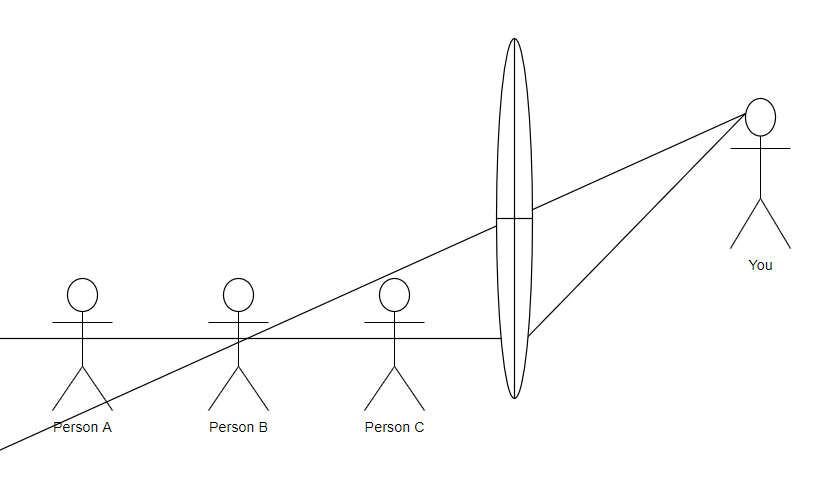
\includegraphics[width=16cm]{diagram.png}
    \end{figure}
\end{center}
As shown in the figure above, all rays passing through this particular lens
for this person converge on Person B so one will get a very clear image of them.
For Person A, and Person C, they will be blurrier as more parts of their body are being
mapped to the same pixel from the (You) perspective.
The ratio determining when the points converge is called the focal length. A key fact
is that the ray that goes through the center of the lens never changes direction \cite{PBR}.
We can use this ray, and the focal length to determine the convergence point and shoot rays
in that direction. To 
get a relatively smooth distribution of points without much aliasing, a Zero-Two sampler was used \cite{PBR}.
Since the lens is a disc, we need a way to convert the $[0, 1)\times[0,1)$ samples from the sampler
to a spherical representation. To achieve this, I used the Box-Muller Transform \cite{weisstein_2020} to
transform it from a uniform distribution to a 2-D normal distribution. While this does lead to bias
for rays around the center of the lens, this effect was not noticeable in the resulting image.
See depth\_of\_field.png, depth\_of\_field\_less.png, depth\_of\_field\_more.png
\subsection{Photon Map - Mapping}
To go about the photon mapping phase, I needed to implement an efficient data
structure to store the spatial data. I choose to go with a kd tree. The algorithm 
for building our photon map attempts to generate some amount of photons per light. This value
was adjusted and tweaked for performance and visual quality. The final result I discovered was effective
and efficient 
was 100000 photons per light. Through the generation process however, this is not exactly the number
of photons generated as some are absorbed or hit pure specular surfaces. Thus a secondary value keeps
track of the actual number of photons added to a running list. At the very end of generation for a light,
the photons are divided by the number of photons generated to get the appropriate light intensity per photon.
I found that tweaking this final intensity by some scalar value helped show photons in low light settings better.
Once this list has been constructed, it is passed to a KD tree which constructs itself based on the points in
this list. The KD tree partitions itself based on a quick-select approach and iterates through
axes per split. When the KD tree is being partitioned, it will perform quick select to partition
the array into two subarrays and create children KD tree nodes with those. This continues until 
the photons in the subarray reach a certain threshold size and a leaf node is added with those photons.
When these photons get added to a leaf node, they create a Bounds, which is essentially an axis aligned bounding box
for the KD Tree node, these will be important for range searching later. Once a child is built and returned, their
bounding box is added to the parent's. This ensures that the parents bounding box always encloses everything it 
has as children. Note that since only $O(n)$ operations are performed at each construction of nodes, where
$n$ is the number of photons, and we separate the tree into two and recurse, by Master's Theorem \cite{cormen_2009}, this construction
is $O(n\log n)$ time. The KDTree is implemented in KDPointTree.hpp/cpp and the Bounds class can be found in Bounds.hpp/cpp.
Photon map can be seen in caustics-map.png
\subsection{Photon Map - Gathering Caustics}
To leverage the photon mapping for caustics, I need to design a high density photon
map which only stores photons that have been specularly reflected/transmitted onto a diffuse object \cite{jensen_1996}.
This means no saving photons unless they are a direct result of a reflection or transmission. The generatePhotons function
in my implementation has an inner loop that loops between 0 and maxDepth number of times, trying to get a photon to go
as far as it can go through reflection and transmission. Note that since there exists only specular reflection and transmission
of rays in my raytracer, this guarantees that after one iteration of the loop, if it has not broken out yet, the photon is being
specularly reflected/transmitted. Thus, when it hits a diffuse surface, we will need to add it to the caustic map. In terms of
actually gathering these we leverage our implementation of range search on the KDTree. The input into the
range search is a point and a radius. Essentially we would like to find is the number of photons inside of that spherical bounds
in the tree. What our range search does is 
approximate the KDTree node as a sphere using the bounding boxes' centroid as the center, and the distance to its max
corner as the radius. This does slightly overfit the bounding volume but its very fast to to test whether or not spheres
overlap. If they do overlap, we recurse on the node until we reach a leaf node. Once we get here, we need to check each point
individually and check if it is actually in the sphere. If it is, we add it to a running list. Ideally, the KDTree is
well balanced and we can eliminate half the photons on each level of recursion. This would give us $O(\log n)$ search
time. In the worst case, the tree is degenerate and we have $O(n)$ search time, where $n$ is number of photons. Once the list
of photons is returned to the gathering function, it checks if it meets a certain size, if not, it will increase the radius
of the search and try again. This was adapted from Jensen's suggestion in \cite{jensen_1996}. 
I add a max radius limit to stop this from becoming to big. Experimentally, I found that $maxRadius=4$ was a good number.
Caustics can be seen in caustics.png
\subsection{Environment Mapping}
As stated in \ref{skybox_ref}, we create a unique object for skyboxes and pass them to the render function. These
are essentially cubes but with the unique feature of having their faces inverted. This means not only are the normals
facing the opposite way, but the UV coordinates go in the opposite way. This allows the skybox textures to be displayed
properly when hit with a ray. A skybox is only tested for collision if there are no other GeometryNode objects to intersect.
When testing for collision, the origin of the ray is always assumed to be zero since we pretend that the skybox
is so far away that the displacement of the ray is negligible. This also guarantees that the ray will intersect the skybox
somehow. Once it intersects, it samples the correct texture and sets the ray colour value to that texture colour.
If a skybox does not exist, the old gradient code is used to make a nice gradient background. See skybox\_test\_no\_sky.png
and skybox\_test\_front.png
\subsection{Modelling}
As part of the modelling objective, I both implemented new primitives: cones and cylinders, and hand modelled some objects.
The implicit equations for the primitives
as well as their partial derivatives for $(u,v)$ are taken from \cite{PBR}. From these, I derived the parametric equations
for intersection as well as the equations for determining $(u,v)$ and the normals. To simplify matters and take advantage of
our hierarchical modelling architecture, the cone is set to a constant height and radius of 1 while the cylinder is 
set to a constant height of 2 and radius of 1. Also, using Blender, I personally hand modelled the potion bottle, pickaxe
and gold ingot. These were exported to .obj files and loaded into the program as Meshes. The Cone and Cylinder
implementations are found in . You can see them in action in the extra\_primitives.png.
\subsection{Final Scene}
The final scene is pretty self explanatory, but there are some technicalities. Firstly, there
are two scripts related to the final scene. One which renders a view of the front of the Minecraft
house with depth of field turned on, anti aliasing on, Phong shading and caustics. The second is a view of the interior
details of the house with anti-aliasing on, caustics, Phong shading but no depth of field. The main reason for this 
was purely aesthetic as I just think the inside looks really nice and would be a shame if it wasn't all visible.
If you look closely you will also see that there is no ceiling. This is also for design aspects since the ender pearl
(green sphere) is highly reflective and looking at it, you can see the part of the house behind the view point as well
as the sky. The final scene script is minecraft.lua and generates screeenshot.png
\section{Extra Features}
You may have noticed that there are some mentions to features not part of the objectives. These 
were simply additional features which I though were must haves during the process that improved the
final result significantly.
\subsection{Phong Shading}
Phong shading is when the normals of a mesh stored at the vertices is interpolated by points on 
a face to find the normal at that point. This leads to smoother meshes that do not look faceted.
To achieve this, what I had to do is compute normals of faces during mesh creation and add them to 
the vertices that it was connected to. Each vertex would then have to keep track of how many normals have
been added to it. After all faces have been process, each vertex will average out the normals and 
save them in a respective vector with the same indices as the corresponding vertex.
 As stated before, Phong shading can be turned on
and off with the CMDArgs. Then, during intersection, we will use the barycentric coordinates obtained by
the Möller–Trumbore algorithm to interpolate the normals using the same indices as the vertices that the
triangles provide. See potion.png and potion-phong.png.
\subsection{Multi-Threading}
I had initially built the raytracer with concurrency in mind, trying my best the avoid 
the use of shared variables that were not read only. This proved to be incredibly useful 
when refactoring the code to achieve concurrency and parallelism. Effectively, the multi-threading process
consists of sending asynchronous calls to the render function and waiting for them all to finish
by the end. The entire image is partitioned into sections and each thread is assigned this section to work on.
The caller of the asynchronous render function will recieve a std::promise that it waits to get resolved after
it finishes calling all the asynchronous calls. The promise returns a vector of tuples. The tuples will include a
position vector and a colour vector. The colour is the colour of that pixel which the raytracer
computed and the position is which image pixel the computed colour should be applied to.
\section{Attributions}
\begin{itemize}
    \item The documentation for Blender was used to help with modelling \cite{foundation_2020}
    \item For the final Minecraft scene, the textures used are taken from the
    Faithful 32x32 Resource Pack \cite{vattic_2020} and altered for use in the raytracer.
    \item The skybox was generated by an online space skybox generator \cite{terrell_2015}.
    \item The (0,2) sampler was taken from \cite{PBR} and adapted for my uses
    \item stb\_image.h \cite{barrett_2020} is used  to load images from disk
    \item The equations definitions for Fresnel reflectance and it's effect on 
    specular reflection/transmission was taken from \cite{PBR}
    \item Photon mapping was improved with suggestions taken from \cite{PBR} and
    \cite{jensen_1996}
    \item \cite{petry_2014} for some normal maps
    \item Many gracious thanks to my parents for keeping me fed during the last nonstop 30+ hours
\end{itemize}

\bibliographystyle{IEEEtran}
\bibliography{references.bib}{}
\end{document}